\chapter{Card Shuffling, Cover Time and Another Glimpse of Randomised Computation}

\section{Card Shuffling}
	Let us now consider a specific class of random processes; that of `shuffling' decks of 
	playing cards (of arbitrary size). Here, we model a deck of cards containing $n$ cards
	as the set $[n]$ defined earlier. Formally, we will think of shuffling the deck as 
	generating a \emph{permutation} $\sigma$ -- that is, a bijection $\sigma \in [n]\rightarrow
	[n]$ -- uniformly at random. We will denote the set of all such permutations $\Sigma_n$.

	\subsection{Strong Stationary Times}
		Before we consider any particular examples of card shuffling, we want to
		introduce a way of telling whether the deck has been shuffled sufficiently. 
		If the method we use to shuffle the deck converges to the uniform distirbution on
		$\Sigma_n$, we might use the mixing time introduced in the last chapter. 
		Alternatively, we introduce the following stopping time.
		\begin{definition}[Strong Stationary Times]
			A stopping time $\tau$ of a Markov chain $(X_t)_{t\in\mathbb{N}_0}$ with
			state space $\mathcal{I}$ and stationary distribution $\pi$ is a 
			\emph{strong stationary time} for the Markov chain if 
			$$
				\forall i,j \in \mathcal{I}.
				\mathbb{P}_i(\tau = t \land X_\tau = j) = \mathbb{P}_x(\tau=t)\pi_j
			$$
			i.e.\ if, when the stopping time has occurred, the Markov chain has reached
			the stationary disribution, regardless of the start state (although the 
			stopping time may be dependent on the starting state).
		\end{definition}

		Now, since such a strong stationary time might be infinite, we would like to 
		provide a bound on the degree of shuffledness at arbitrary times.
		\begin{lemma}
			If $(X_t)_{t\in\mathbb{N}_0}$ is a Markov chain over state space $\mathcal
			{I}$ with stationary 
			distribution $\pi$, and strong stationary time $\tau$, then 
			$$
				\forall i \in \mathcal{I}, t\in\mathbb{N}_0.
				\|\mathbf{p}_x^t-\pi\|_{tv} \leq \mathbb{P}_x(\tau > t).
			$$
		\end{lemma}
		\begin{proof}
			We have that, if $I \subseteq \mathcal{I}$, then
			\begin{align*}
				&\mathbb{P}_x(X_t \in I) - \pi(I) \\
				=& \mathbb{P}_(X_t \in I | \tau > t)\cdot\mathbb{P}_x(\tau > t) 
				+\mathbb{P}_x(X_t \in I |\tau \leq t)\cdot\mathbb{P}_x(\tau \leq t)
				-\pi(I) \\
				=&(\mathbb{P}_x(X_t\in I|\tau>t)-\pi(I))\cdot\mathbb{P}_x(\tau>t)\\
			\end{align*}
			Then, since $\mathbb{P}_x(X_t\in I|\tau>t)-\pi(I))\in[-1,1]$, we have that
			\begin{align*}
				|\mathbb{P}_x(X_t \in I) - \pi(I)| &=  
				|(\mathbb{P}_x(X_t\in I|\tau>t)-\pi(I))|\cdot\mathbb{P}_x(\tau>t)\\
				&\leq \mathbb{P}_x(\tau>t).
			\end{align*}
			By lemma \ref{lemma:tvsup}, and since this holds for any $I$, we complete 
			the proof by taking the supremum on both sides.
		\end{proof}


	\subsection{Top-to-Random Shuffling}
		The first method of shuffling we now consider is that of \emph{top-to-random} (TTR) 
		shuffling, in which the top card of the deck is removed and replaced into the deck
		at a position chosen uniformly at random.\par
		Formally, we can model this as a Markov chain $(\varsigma_t)_{t\in\mathbb{N}_0}$ 
		over the state space $\Sigma_n$, in 
		which the transition matrix $\mathbf{P}$ is given by
		$$
			P_{\sigma_1, \sigma_2} = 
			\begin{dcases}
				\frac{1}{|A_{\sigma_1}|} = \sfrac{1}{n} 
				& \sigma_2 \in A_{\sigma_1} \\
				0 & \sigma_2 \notin A_{\sigma_1}
			\end{dcases}
		$$
		where we define $A_{\sigma_1} \subset \Sigma_n$ to be the set of permutations 
		`adjacent'\footnote{In the sense that we only have to move one card to move between 
		the permutations} 
		to $\sigma_1$, that is $A_{\sigma_1} \coloneqq \{\sigma\in\Sigma_n
		: \exists i \in [n]. \forall j \in [n] . (j < i \implies \sigma(j)=\sigma_1(j+1))
		\land (j = i \implies \sigma(j) = \sigma_1(0)) \land (j > i \implies \sigma(j)=
		\sigma_1(j))\}$.\par
		It should be reasonably clear that if $\sigma \in A_\rho$, then $\rho \in
		A_\sigma$, and that the chain is irreducible since any permutation can be reached 
		from any other. Therefore, the chain has a unique stationary distribution, which is
		the uniforma distribution over $\Sigma_n$ since all transition probabilities are 
		equal. Since any permutation is also accessible in one time step from 
		itself, the chain is aperiodic, and therefore converges to stationarity, as 
		desired. \par
		Let us now provide an example of a strong stationary time for the TTR shuffle. 
		We define $\tau_\top \coloneqq \inf(t\in\mathbb{N}_0:\varsigma_{t-1}(0)
		= \varsigma_{0}(n-1))$, i.e.\ the time step immediately after the card that was 
		originally on the bottom of the deck was first on the top. Thus,
		\begin{claim}
			$\tau_\top$ is a strong stationary time for the TTR shuffle.
		\end{claim}
		\begin{proof}
			We have already discussed that the stationary distribution for the TTR is
			indeed the uniform distribution over $\Sigma_n$. Thus we will prove this
			claim by showing that, for any time $t$, the cards under $\varsigma_0(n-1)$
			are arranged in an order that was sampled from a uniform distribution of 
			their permutations.\\
			To this end, we proceed by induction over $t$, and note that the base case 
			holds because at $t=0$, there is only one possible permutation of the cards
			below $\varsigma_0(n-1)$, since there are none.\\
			Suppose now that the claim holds for some $t \in\mathbb{N}_0$, and let the 
			number of cards below $\varsigma_0(n-1)$ be $k\in\mathbb{N}_0$. Then any 
			one of the permutations of the cards below the original bottom card is 
			equally likely by assumption, so if $\varsigma_{t+1}^{-1}(\varsigma_{t}(0))
			< \varsigma_{t+1}^{-1}(\varsigma_{0}(n-1))$, then the cards below the 
			original bottom card remain uniformly sampled. Otherwise, the card at the 
			top of the deck at $t$ is placed below $\varsigma_0(n-1)$, uniformly at 
			random at any one of the $k+1$ possible positions it could go to, so 
			the new permutation is still chosen at random from the now $(k+1)!$ 
			possibilities.\\
			Therefore, if $\tau_\top\downarrow$, then at $\tau_\top -1$, the
			bottom card of the first permutation will have moved to the top, so
			all other cards will be permuted unifomrly at random. The shuffle will have
			reached complete uniformity in its distribution when then that card is
			placed at a new location in the deck.
		\end{proof}
		\par

		At the moment, however, we have little indication of how large $\tau_\top$
		may be. Therefore, we will also consider the mixing time for the TTR shuffle to
		gain an idea of how quickly the TTR shuffle approaches uniformity. In fact,
		\begin{lemma}
			When applying the top-to-random shuffle to a deck of $n$ cards, for any 
			$\epsilon \in \mathbb{R}^+$, $\tau(\epsilon) \in O(n \log n)$. 
		\end{lemma}
		\begin{proof}
			Suppose that a card has just been placed underneath the card that was 
			originally at the bottom, and that there are now $k-1$ cards under it.
			Then at any time step before the $k$th card is placed beneath it, the 
			probability that this will happen in the next time step is $\sfrac{k}{n}$,
			which is the same probability as that of reducing the number of empty from
			$k$ to $k-1$ at any given time step in the `balls into bins' experiment 
			discussed in Chapter 1. Therefore, the probability that, within 
			$n \ln n + Cn$ time steps, we have increased the number of cards below the
			original bottom card from $0$ to $n-1$ is the same as that of gowing from 
			$n$ empty bins to $0$ in the balls into bins experiment, which we had 
			earlier shown to be $\geq 1 - e^{-C}$. Therefore, if we take $C \geq -\ln 
			\epsilon$ we obtain the result.
		\end{proof}
		Note that, with this result, we can approximate the speed at which we reach an 
		approximately uniform distribution is roughly $t_\mathrm{mix}\approx\ln|\Sigma_n|$.

		\subsection{Riffle Shuffling}
		The above method of shuffling a deck of cards is rather artificial. When we shuffle 
		deck of cards in real life, we mostly use a method of shuffling known as `riffle 
		shuffling', which we shall model mathematically as follows:
		\begin{enumerate}[(1)]
			\item Split the deck into two piles, the sizes original of which are 
			$(l_0, n-l_0)$ where $l_0 \sim \mathrm{Bin}(n, \sfrac{1}{2})$.
			\item Generate a new permutation of $[n]$ by adding the bottom card of 
			one of the stacks, where the first stack is chosen with probability 
			$\frac{l}{l+r}$, where $l$ and $r$ are the remaining sizes of the two 
			stacks, respectively. 
		\end{enumerate}
		
		It can be shown (though we will not do so) that for this model of shuffling, we 
		have $t_\mathrm{mix} \leq 2 \log_2(n\cdot\sfrac{4}{3})$. Note also that this 
		means the riffle shuffle is essentially exponentially quicker than the TTR shuffle, 
		as here $t_\mathrm{mix} \approx \ln\ln |\Sigma_n|$. 

		Historically, this result was reached by Dave Bayer and Persi Diaconis, who in 
		their paper `Trailing The Dovetail Shuffle To Its Lair' also present the
		data for shuffling various size decks of cards presented in table 
		\ref{table:bayer}, which has led to the common claim
		that `seven riffle shuffles are enough'.  \par
		As the reader can see, this claim is not grounded in any actual fact, at least not 
		if we take our usual definition of $t_\mathrm{mix} \coloneqq \tau(\sfrac{1}{4})$.
		The 
		claim, historically, arose since, for a 52-card deck, the total variation distance,
		taken as an inverse measure of `shuffledness', is reasonably stationary up to the 
		seventh riffle shuffle, whereas it roughly halves after every subsequent iteration 
		of the shuffle, meaning that at seven shuffles, `the deck starts being truly 
		shuffled'.
%
		\begin{center}
			\begin{table}
				\caption{The total variation distance of the distribution over 
				the permutations of $m$ cards after $t$ iterations of the riffle 
				shuffle.}
				\vspace{1em}
				\label{table:bayer}
				\begin{tabular}{C{0.825cm}C{0.825cm}C{0.825cm}C{0.825cm}C{0.825cm}
				C{0.825cm}C{0.825cm}C{0.825cm}C{0.825cm}C{0.825cm}C{0.825cm}}
				\hline
				$m$&1&2&3&4&5&6&7&8&9&10\\
				\hline
				25&1.000&1.000&0.999&0.775&0.437&0.231&0.114&0.056&0.028&0.014\\
				32&1.000&1.000&1.000&0.929&0.597&0.322&0.164&0.084&0.042&0.021\\
				52&1.000&1.000&1.000&1.000&0.924&0.614&0.334&0.167&0.085&0.043\\
				78&1.000&1.000&1.000&1.000&1.000&0.893&0.571&0.307&0.153&0.078\\
				104&1.000&1.000&1.000&1.000&1.000&0.988&0.772&0.454&0.237&0.119\\
				208&1.000&1.000&1.000&1.000&1.000&1.000&1.000&0.914&0.603&0.329\\
				312&1.000&1.000&1.000&1.000&1.000&1.000&1.000&0.999&0.883&0.565
				\end{tabular}
			\end{table}
		\end{center}

\section{Cover Time}
	We now turn our attention with more focus to the concept of \emph{random walks}, introduced
	in Chapter 2. In particular, we will consider the \emph{cover time} of random walks over
	graphs, which measure the number of time steps it takes for the random walk to have 
	`visited' each vertex of the graph. Formally, we define the cover time as follows.
	\begin{definition}[Cover Time]
		Suppose that $G = (V, E)$ is a connected, finite, undirected graph and that 
		$(X_t)_{t\in\mathbb{N}_0}$ is some random walk over $G$. Then the \emph{cover 
		time} of $G$ under $(X_t)_{t\in\mathbb{N}_0}$ $t_{\mathrm{cov}, X}(G)$ is given by 
		$$
			t_{\mathrm{cov}, X}\coloneqq \lambda (V, E) .
			\max_{v\in V}\mathbb{E}_v(\tau_\mathrm{cov},X)
			\text{\ \ \ where\ \ \ }
		      \tau_{\mathrm{cov},X}\coloneqq\inf\left(t:\bigcup_{i=0}^{i=t}\{X_t\}=V\right)
		$$
		When the random walk is the simple random walk over the graph, we omit the 
		indication of which random walk is being considered. We will only consider the 
		SRW throughout this section.
	\end{definition}
	For example, consider the following random walk over the graph presented below, where
	the random walk steps through $t$, $u$, $t$, $w$, $v$ over the course of the first four 
	time steps, so that $\tau_\mathrm{cov} = 4$. 
	\begin{center}
	       	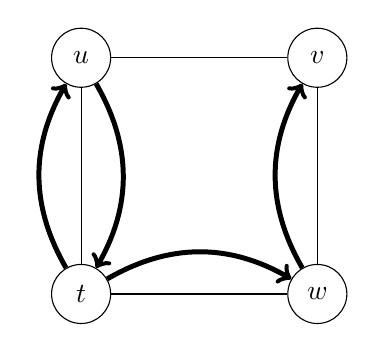
\begin{tikzpicture}
	       		\draw node[circle, draw, minimum size=0.75cm] (i) {$t$};
	       		\draw node[circle, draw, minimum size=0.75cm] 
	       		[above of=i, node distance=3cm] (j) {$u$};
	       		\draw node[circle, draw, minimum size=0.75cm] 
	       		[right of=j, node distance=3cm] (k) {$v$};
	       		\draw node[circle, draw, minimum size=0.75cm] 
	       		[right of=i, node distance=3cm] (l) {$w$};
	       		\draw[->, line width=1.8pt] (i) edge [bend left] (j);
	       		\draw[->, line width=1.8pt] (j) edge [bend left] (i);
	       		\draw[->, line width=1.8pt] (i) edge [bend left] (l);
	       		\draw[->, line width=1.8pt] (l) edge [bend left] (k);
	       		\draw[-] (j) edge (i);
	       		\draw[-] (j) edge (k);
	       		\draw[-] (l) edge (i);
	       		\draw[-] (k) edge (l);
	       		\draw[-] (l) edge (k);
	       	\end{tikzpicture}
	\end{center}

	Before we move on to bound the cover time, we must first establish the stationary 
	distribution of the simple random walk, as it will be helpful throughout this section.
	Hence,
	\begin{lemma}
		\label{lemma:srwstat}
		Suppose $(X_t)_{t\in\mathbb{N}_0}$ is the simple random walk over a connected,
		undirected graph $G = (V,E)$, with transition matrix $\mathbf{P}$. Then, 
		the unique stationary distribution $\pi$ of $(X_t)_{t\in\mathbb{N}_0}$, the 
		existence of which is guaranteed by theorem \ref{theorem:uniquestationary},
		is given by $\pi \coloneqq \left(\frac{d(v)}{2|E|}\right)_{v \in V}$.
	\end{lemma}
	\begin{proof}
		Firstly, we note that quite clearly, $\sum_{v\in V} \pi_v = 1$; that is, $\pi$
		is indeed a probability distribution. \\
		Secondly, $\pi$ has the desired eigenvector property since
		\begin{align*}
			(\pi\cdot\mathbf{P})_v &= \sum_{u \in V} \pi_u P_{u,v} \\
			&= \sum_{u\in V} \frac{d(u)}{2|E|} P_{u,v} \\
			&= \sum_{u:\{u,v\}\in E} \frac{d(u)}{2|E|} \cdot \frac{1}{d(u)} \\
			&= \frac{d(v)}{2|E|} = \pi_v
		\end{align*}
		for any $v \in V$. Since theorem \ref{theorem:uniquestationary} guarantees 
		uniqueness, this completes the proof.
	\end{proof}
	We further present the \emph{crossing time} of an edge, the expected time before an edge of
	the graph has, effectively, been crossed, that is, until one of its endpoints has been 
	reached after starting at the other. To be precise:
	\begin{lemma}
		\label{lemma:srwhit}
		If $G=(V,E)$ is a connected, finite, undirected graph, and $\{u,v\} \in E$, then 
		for the SRW over $G$, $h_{u,v} \leq 2|E|$.
	\end{lemma}
	\begin{proof}
		Note that from the result in lemma \ref{lemma:srwstat}, we can obtain 
		$$
			\mathbb{E}_v(\tau^+) = \sfrac{1}{\pi_v} = \frac{2|E|}{d(v)}.
		$$
		We also obtain, by the Markov Property, that 
		$$
			\mathbb{E}_v(\tau^+) = 1 + \sum_{w : \{v,w\}\in E} \frac{h_{w,v}}{d(v)}
		$$
		We combine these results to obtain, if $\{u, v\} \in E$,
		\begin{align*}
			h_{u,v} &\leq \sum_{w : \{v,w\}\in E} h_{w,v}\\
			&= d(v) \cdot \left(\frac{2|E|}{d(y)} - 1\right) \\
			&\leq 2|E|
		\end{align*}
	\end{proof}

	Now, we can make a statement about the cover time of the SRW over graph $G$, which will
	allow us to draw helpful conclusions about a probabilistic algorithm we will introduce at
	a later time.
	\begin{lemma}
		\label{lemma:srwtcov}
		If $G = (V, E_G)$ is a connected, undirected graph, then the cover time of the 
		simple random walk over $G$ has 
		$$
			t_\mathrm{cov}(G) \leq 4n \dot |E| \leq 2n^3
		$$
		where $n = |V|$.
	\end{lemma}
	The proof of this lemma relies on the following fact:
	\begin{claim}
		If $G = (V, E_G)$ is a connected, undirected graph of $n\in\mathbb{N}$ vertices, 
		then there exists a tree $T = (V, E_T)$ that spans the vertices of $G$, such that 
		$E_T \subseteq E_G$ and $|E_T| = n-1$.
	\end{claim}
	\begin{proof}
		We proceed by (strong) induction on $n$. If $n = 1$, then $T$ is just given by $G$.
		\\\ \\
		Now suppose that this claim holds for all integers $i \leq n$ for some $n$. Then
		suppose that graph $G = (V,E_G)$ has $n+1$ vertices. If we now fix some $v \in V$
		and consider the graph that results from removing $v$ from $G$, this graph will 
		be partitionable in some number $k$ of connected subgraphs that are not 
		interconnected, each of which will have strictly fewer than $n+1$ vertices.
		\\
		That is, each of the $k$ subgraphs will have a spanning tree $T_i = (V_i, E_i)$ 
		of $n_i - 1$ 
		edges, where $n_i$ is the number of vertices in subgraph $i$. Then, since $G$ is 
		connected, and none of the $k$ subgraphs are interconnected, we know that $\forall
		i. \exists u \in V_i . \{u, v\} \in E_G$. Fix one such $u$ for each subgraph, and 
		construct $T=(V, \bigcup_i (E_i \cup \{u_i, v\}))$, then $T$ will be a spanning 
		tree over $G$, and have $|E_T| = \sum_i |E_i| + 1 = \sum_i |V_i| - 1 +1 = |V|-1$,
		as desired.
	\end{proof}
	We can now proceed with the proof of the lemma.
	\begin{proof}[Proof of lemma \ref{lemma:srwtcov}]
		Consider a spanning tree $T$ for the graph $G$, with the properties described in 
		the above claim. Then fix some vertex $v_0 \in V$, and fix a `tour' $(v_i)_{i=0}^
		{i=2n-2}$ on the tree that visits all vertices of the graph, and returns to $v_0$
		\footnote{Since $T$ is a tree, this will be a DFS on $T$ that then walks back up 
		to $v_0$.}. \\
		The cover time of $G$ under the SRW is at most the time it will take to visit the 
		vertices of the tour in the right order in the SRW, from the worst case $v_0$. That
		is,
		\begin{align*}
			t_\mathrm{cov} &\leq \sum_{i=0}^{i=2n-3} h_{v_i, v_{i+1}} \\
			&=\sum_{\{u,v\}\in E_T} h_{u,v} + h(v,u) \\
		\intertext{Observe now that for any edge $\{u,v\} \in E_G$, we have that $h_{u,v} 
		\leq 2\cdot|E|$ by lemma \ref{lemma:srwhit}.}
			&\leq 2 \cdot \sum_{\{u,v\}\in E_T} 2 |E_G| \\
			&\leq 4n \cdot |E|
		\end{align*}

		The second part of the lemma follows from the fact that in any undirected graph
		of $n$ vertices, there are at most $(n^2 - n)/2$ edges.
	\end{proof}

	It is actually possible to obtain a tighter bound for the cover time of connected graphs 
	under the SRW, the following result is known as the Matthews bound (after Peter Matthews,
	who published the result in 1986).
	\begin{theorem}[Matthews Bound]
		If $G =(V,E)$ is a connected, undirected graph, then for the simple random walk 
		over $G$, we have that
		$$
		t_\mathrm{cov}(G) \leq \left(\sum_{i=1}^{i=n-1} \sfrac{1}{i}\right) \approx
		\ln(n) \cdot \max_{u,v\in V}(h_{u,v})
		$$
	\end{theorem}
	We will not prove the Matthews bound, as its proof is somewhat lengthy and certainly not 
	trivial. However, the reader should note that the proof does not rely on any material not 
	yet presented in these notes. As such, we refer (for the original proof), to Peter 
	Matthews (1986): `Covering Problems for Brownian Motion on Spheres', Section 2.

	\subsubsection{SRW Over A Path}
	Let us now consider a particular example, that of conducting the SRW over the 
	$n$-\emph{path} $P_n$ of $n$ edges. We define this graph to be $P_n\coloneqq([n+1],E_P)$, 
	where $E_P \coloneqq \{\{u,v\} \subseteq [n+1] : |u-v| = 1\}$.
	
	We will bound the cover time of the $n$-path to within a constant factor. To this end, we 
	we require the following result.
	\begin{claim}
		For the SRW over $P_n$, for any $k \in [n+1]$, $h_{k,n} = n^2-k^2$.
	\end{claim}
	\begin{proof}
		Denote $h_{k,n}$ as $f_k$, and notice that $f_n = 0$. By the Markov property, we
		have that $f_0 = 1 + f_1$, and 
		$$
			f_k = 1 + \frac{f_{k-1}}{2} + \frac{f_{k+1}}{2}
		$$
		for all other $1 \leq k \leq n-1$. This forms a system of $n$ equations, with $n$ 
		unknowns, so there is a \emph{unique} solution. That is, if the solutions 
		$f_k = n^2-k^2$ satisfies the equations, they are the correct solutions. Indeed,
		for any $0 \leq k < n$, it is easy to verify that the equations become satisfied.
		\\
		The proof is completed by noticing that $f_n = 0 = n^2-n^2$.
	\end{proof}

	From this result, we can bound the cover time of $P_n$ fairly straightforwardly. This 
	result is stated in lemma \ref{lemma:pathcovt}.
	\begin{lemma}
		\label{lemma:pathcovt}
		For the $n$-path $P_n$, we have 
		$$
			n^2 \leq t_\mathrm{cov}(P_n) \leq 2n^2
		$$
	\end{lemma}
	\begin{proof}
		The lower bound is obtained by noticing that, if the starting vertex is either one 
		of the end points of $P_n$, then the expected time to cover the graph will be the 
		expected time to reach the other end point, i.e.\ $h_{0,n} = h_{n,0} = n^2$. \\
		For the upper bound, notice that regardless of where we start, we expect to reach 
		one of the end points in at most $n^2$ steps, from where we expect to reach the 
		other in exactly $n^2$ steps, covering the entire path in the process.
	\end{proof}

\section{Randomised Computation}
	This section will firstly classify different kinds of randomised algorithms, and then 
	consider two examples of randomised approximation algorithms for well-known decision 
	problems that have certain benefits over their deterministic counterparts.

	\subsection{Different Classes of Randomised Computation *}
	We will first consider algorithms designed merely for decision problems. Intuitively, one 
	simple kind of randomised algorithm might be one that makes decisions based on some 
	probability distribution, but guarantees a result to be found. This is an informal way to 
	define \emph{Las Vegas algorithms}. Formally, we define them as follows:
	\begin{definition}[Las Vegas Algorithm]
		Given a decision problem $L \subseteq \Sigma^*$, an algorithm $A$ operating on 
		$\Sigma^*$ is a Las Vegas Algorithm for $L$ if, for any $x \in \Sigma^*$, if
		$A$ reaches a conclusion about $x$, then this conclusion is correct, that is,
		$A(x) = \text{``yes''} \iff x \in L$. Notice that such an algorithm does not have
		to come to a conclusion, it can halt informing of failure to reach a conclusion.
	\end{definition}
	\begin{comment}
		It is important to note that the class of Las Vegas algorithms makes no guarantees
		about the run time given a certain instance of a problem; in fact the run time of 
		a Las Vegas Algorithm $A$ on any $x \in \Sigma^*$ is a random variable $RT_{A, x}$.
	\end{comment}

	The consideration of Las Vegas algorithm run times gives way for a further subdivision of 
	this class of randomised algorithm---based on an algorithm $A$'s \emph{completeness}, as 
	defined below.
	\begin{definition}
		A Las Vegas Algorithm $A$ is \emph{complete} if there exists a $t_\mathrm{max} 
		\in \mathbb{N}$ such that, for any soluble $x \in \Sigma^*$, $\mathbb{P}(RT_{A,x} 
		\leq t_\mathrm{max}) = 1$.\\
		It is \emph{almost complete} if, for any soluble $x \in \Sigma^*$, $\lim_{t
		\rightarrow\infty}\mathbb{P}(RT_{A, x} \leq t) = 1$. It is \emph{essentially 
		incomplete} when it is neither complete nor almost complete.
	\end{definition}
	\par
	A class of randomised algorithms that \emph{does} make a guarantee about the algorithm 
	run time is that of \emph{Monte Carlo algorithms}, which instead makes a concession about 
	the correctness of any conclusion the algorithm comes to. Their formal definition is:
	\begin{definition}[Monte Carlo Algorithm]
		For some decision problem $L \subseteq \Sigma^*$, an algorithm $A$ operating on
		$\Sigma^*$ is a Monte Carlo algorithm for $L$ if $A$ reaches a conclusion about
		any $x \in \Sigma^*$, where the truth value of the conclusion is distributed 
		according to some probability distribution $\Pr_x$.
	\end{definition}
	The class of Monte Carlo algorithms may also be further partitioned, here we commonly 
	consider whether the error probabilities are \emph{one-} or \emph{two-sided}. 
	An algorithm has one-sided error if one decision outcome (``yes'' or ``no'') is always 
	correct, while the other may be incorrect. Algorithms with two-sided errors may 
	come to incorrect conlcusions either way. \\
	Different subclasses of the Monte Carlo algorithms include:
	\begin{definition}[RP and co-RP Algorithms]
		An algorithm $A$ over $\Sigma^*$ is RP (randomised polynomial time) if, if there 
		exists a $t \in \mathbb{R}^+$, such that for any $x \in \Sigma^*$, it halts 
		within polynomial time, and we have
		\begin{itemize}
			\item $x \notin L \implies A(x) =$ ``no'', and
			\item $x \in L \implies \mathbb{P}(A(x) = \text{``yes''}) \geq t$.
		\end{itemize}

		$A$ is a co-RP algorithm if it is an RP algorithm for $\Sigma^* \setminus L$.
	\end{definition}
	\begin{comment}
		(co-)RP algorithms are examples of algorithms with one-sided error. \\
		This means that we can draw the following useful conclusion about certain 
		outcomes of an RP $A$: If $x \notin L$, then the answer will be correct, and 
		contrapositively, if the conclusion of $A$ is ``yes'', then it is also correct.
	\end{comment}
	\begin{definition}[BPP Algorithms]
		An algorithm $A$ operating on $\Sigma^*$ is BPP (Bounded-error Probabilistic 
		Polynomial Time) if $\exists \epsilon \in \mathbb{R}^+$ such that $A$ halts in 
		polynomial time on any instance $x \in \Sigma^*$, and for any soluble instance $x
		$ comes to the correct conclusion with probability at least $\sfrac{1}{2} + 
		\epsilon$.
	\end{definition}
	\begin{comment}
		One sometimes sees BPP defined as the class of algorithms that conlcude 
		incorrectly with probability at most $p < \sfrac{1}{2}$, where $p$ is some fixed 
		constant. It should be noted, however, that for any choice of $p$, the generated 
		class of algorithms remains the same. This is why we present the more general 
		form as above.
	\end{comment}

	We should also mention those probabilistic algorithms for computation problems. We have 
	already seen a few examles of these, such as the RandMaxCut algorithm in Section 1.3, or 
	the well-known Bucket Sort algorithm taught in IA algorithms, and mentioned in the 
	Introduction. We commonly divide computation algorithms into \emph{exact} algorithms, 
	that return an exact value for the problem they address, and \emph{approximation} 
	algorithms, which approximate the correct results. Of course, Bucket Sort is an example 
	exact algorithm, while RandMaxCut is an approximation algorithm. \par
	In fact, algorithms that exhibit a one-sided error, such as RandMaxCut, lend themselves 
	to a technique known as \emph{amplification}; in which the accuracy of the approximation, 
	or the correctness of a decision is improved by repeating the execution of the algorithm. 
	We will soon see another example of an algorithm susceptible to amplification, a 
	randomised algorithm for deciding \emph{s-t-reachability}.

	\subsection{$s$-$t$-Reachability}
	The first decision problem for which we will consider a randomised algorithm is that of 
	$s$-$t$-Reachability. Recall that this decision problem is that of, given an undirected 
	finite graph $G =(V,E)$, and two of its vertices, $s$ and $t$, deciding whether there is a 
	path $v_0, v_1, \hdots v_n$ such that $\forall 0 \leq i < n. \{v_i , v_{i+1}\} \in E \land
	v_0 = s \land v_n = t$, and that this problem is solvable either in nondeterministic 
	logarithmic space (i.e.\ square-logarithmic deterministic space), or deterministic 
	polynomial time, but in the former case, the run time of the deterministic algorithm 
	becomes inefficient, whereas in the latter case the algorithm requires linear space. 
	\par
	Therefore, we introduce the following algorithm:
	\begin{lstlisting}[label=listing:streach, caption={Randomised $s$-$t$-Reachability},
	style=mystyle]
def st_reach(G, s, t):
     srw(G, start_vertex=s, run_time=4*size(G.V)^3, mark_visited=True)
     return t.visited
	\end{lstlisting}
	In case the pseudocode is not clear enough, the algorithm conducts a SRW over the graph $G$
	for at most $4|V|^3$ time steps, and concludes that $t$ is reachable from $s$ if it is 
	ever visited by that SRW. Clearly, this algorithm runs in $O(n^3)$ time for a graph of $n$ 
	vertices, and only uses lograithmic space---it is very similar to the common 
	nondeterministic logspace algorithm for $s$-$t$-Reachability. Of course,  the conclusion 
	reached by this algorithm may be incorrect---crucially, though, this algorithm exhibits a 
	one-sided error. In fact, it is an example of an RP algorithm, since if $s \not\leadsto t
	$ the SRW starting at $s$ will never reach $t$, but there is a positive probability that 
	if $s \leadsto t$\footnote{We use this notation to indicate that there is a path between $
	s$ and $t$.}, then the algorithm will decide ``yes''. This probability can be bounded to 
	be at least $\sfrac{1}{2}$, as presented below.
	\begin{lemma}
		\label{lemma:srwreachampl}
		If $G = (V, E)$ is an undirected graph such that for $s, t \in V$, $s \leadsto t$,
		then $\mathbb{P}(\mathtt{st\_reach}(G, s, t) = \mathtt{True}) \geq \sfrac{1}{2}$.
	\end{lemma}
	\begin{proof}
		Assuming that $s \leadsto t$, let $G' = (V', E')$ be the connected component of 
		the graph that they are members of. Then we have that
		\begin{align*}
			\mathbb{P}(\mathtt{st\_reach}(G, s, t) = \mathtt{True}) &\geq 
			\mathbb{P}_s(\tau_\mathrm{cov}(G') \leq 4 |V|^3) \\
			&\geq\mathbb{P}_s(\tau_\mathrm{cov}(G')\leq4|V'|^3)
			&\text{by the tail bound}\\
			&\geq 1 - \frac{\mathbb{E}_s(\tau_\mathrm{cov}(G'))}{4|V'|^3}&
			\text{by Markov's inequality}\\
			&\geq 1 - \frac{t_\mathrm{cov}(G')}{4|V'|^3} \\
			&\geq \sfrac{1}{2}
		\end{align*}
	\end{proof}
	Now, clearly, this means that the algorithm \texttt{st\_reach} lends itself to 
	amplification, since we can run it $N$ times to obtain a decision with at error 
	probability of at most $2^{-N}$, while remaining in cubic time.

	\subsection{Boolean Satisfiability}
	The next class of problems we will consider is perhaps the most well-studied class of 
	decision problems in Complexity Theory, that of \emph{boolean satisfiability}, or \textsc{
	Sat}. We will only consider the subset of instances \textsc{Sat} which are formul\ae\ in 
	\emph{conjunctive normal form} (CNF), that is, we will focus on \textsc{CNF-Sat}. In 
	particular, we will consider the even more restricted special case of 2-\textsc{Sat}, the 
	problem where each clause comprises exactly two literals. Recall that (any special case of)
	\textsc{Sat} is generally speaking NP-hard, whilst \emph{\textsc{Sat}-solvers} are 
	extremely commonly used to solve general NP problems efficiently; this is a result of many 
	optimisation techniques involving solving heuristics, etc. We will explore a way of 
	efficiently deciding instances of 2-\textsc{Sat} and, should the instance be satisfiable, 
	returning a correct solution.\\
	To clear up some terminology, an instance of 2-\textsc{Sat} is a formula $\phi$ in 2-CNF, 
	comprising variables from an enumerable set $\mathbb{X} \coloneqq \{x_i : i \in \mathbb{N
	}\}$. Should the instance be satisfiable, a solution to it is a partial function $\theta 
	\in \mathbb{X} \rightharpoonup \mathbb{T}$, where $\mathbb{T}$ is the set of truth values, 
	$\mathbb{T} \coloneqq \{\top,\bot\}$, such that $[\theta]\phi$ (the substitution $\theta$ 
	applied to $\phi$) reduces to $\top$. \par
	We will discuss the algorithm presented in listing \ref{listing:rand2sat}.
	\begin{lstlisting}[label=listing:rand2sat, caption={A randomised algorithm for 
	2-\textsc{Sat}}, style=mystyle]
def rand2Sat(phi):
    variables = set(vars(clause) for clause in phi)
    n = size(variables)
    solution = {v : False for v in variables}
    repeat n^2 times:
        if solution.satisfies(phi):
            return solution
        v = phi[phi.apply(solution) != True].randomClause().randomVariable()
        solution[v].flip()
    raise UnsatisfiableError
	\end{lstlisting}
	Before we go on to analyse this algorithm more carefully, we introduce some terminology.
	Let us call each iteration of the loop beginning on line 5 a \emph{step}, then let 
	$\theta_i$ be the variable assignment at step $i$. If now the formula $\phi$ happens to be 
	satisfiable, fix some solution $\vartheta$ (and suppose that the range of $\vartheta$ is 
	the same as that of any $\theta_i$; the set of variables occuring in any clause of $\phi$) 
	and let $\Delta_i\coloneqq|\{x\in\mathrm{range}(\vartheta):\theta_i(x)=\vartheta(x)\}|$.
	\par
	Now we determine the expected number of steps that need to be taken before, for a 
	satisfiable formula $\phi$, a correct solution $\theta$ is found. Obviously, for an 
	unsatisfiable formula, this will never occur, so the algorithm will decide ``no'' with 
	probability 1. 
	\\
	So,
	\begin{claim}
		If, for an instance $\phi$ of 2-\textsc{Sat}, a correct solution $\theta$ exists, 
		then the expected number of steps the randomised algorithm presented in listing 
		\ref{listing:rand2sat} makes is at most $n^2$, where $n$ is the number of distinct 
		variables occuring as literals in $\phi$.
	\end{claim}
	\begin{proof}
		Fix some particular such solution $\theta$, then notice that 
		\begin{enumerate}[(1)]
			\item $\mathbb{P}(\Delta_{i+1} = 1 | \Delta_i = 0) = 1$,
			\item $\mathbb{P}(\Delta_{i+1} = k+1 | \Delta_i = k) \geq \sfrac{1}{2}$,
			\item $\mathbb{P}(\Delta_{i+1} = k-1 | \Delta_i = k) \leq \sfrac{1}{2}$.
		\end{enumerate}
		We also note that $\Delta_i = n \iff \theta_i = \theta$, so if such an $i$ occurs,
		the algorithm returns a correct solution in at most $i$ steps; some other correct 
		solution may have been found at step $j < i$. \\
		Now, in the worst case, we have $\Delta_0 = 0$. With (1)-(3), it is possible 
		(though the details of this are ommitted here) to couple $(\Delta_i)_{i\in
		\mathbb{N}_0}$ with the SRW $(W_i)_{i\in\mathbb{N}_0}$ on the $(n-1)$-path such 
		that, if $T$ is the number of steps to find a correct solution, then 
		$$
			\mathbb{E}(T) \leq \mathbb{E}_0(\inf(t : \Delta_t = n)) 
			\leq  \mathbb{E}_0(\inf(t : W_t = n)) 
			= h_{0,n} = n^2
		$$
	\end{proof}
	From this, similarly to the result of lemma \ref{lemma:srwreachampl}, we may obtain 
	lemma \ref{lemma:randsatampl}.
	\begin{lemma}
		\label{lemma:randsatampl}
		For a satisfiable instance $\phi$ of 2-\textsc{Sat}, the randomised algorithm 
		presented in listing \ref{listing:rand2sat} returns a correct solution in time 
		$2n^2$ with probability at least $\sfrac{1}{2}$.
	\end{lemma}
	From this result, it follows straightforwardly that this algorithm, too, is suitable for 
	amplification, such that we can obtain an arbitrarily low error probability within 
	quadratic time with respect to the input size.
